
\item A caixa tem massa de \SI{150}{\kilogram} e repousa em uma superfície para a qual os coeficientes de atrito estático e cinético são $\mu_{s}=0.3$ e $\mu_{k}=0.2$, respectivamente. Se o motor $M$ fornece uma força no cabo $F=(8\,t^{2}+20)\,$\SI{}{\newton}, onde $t$ é dado em segundos, determine a potência de saída desenvolvida pelo motor quando $t=\SI{5}{\second}$.

\import{answers/}{answer-9}

\vspace{7cm}
\begin{flushleft}
    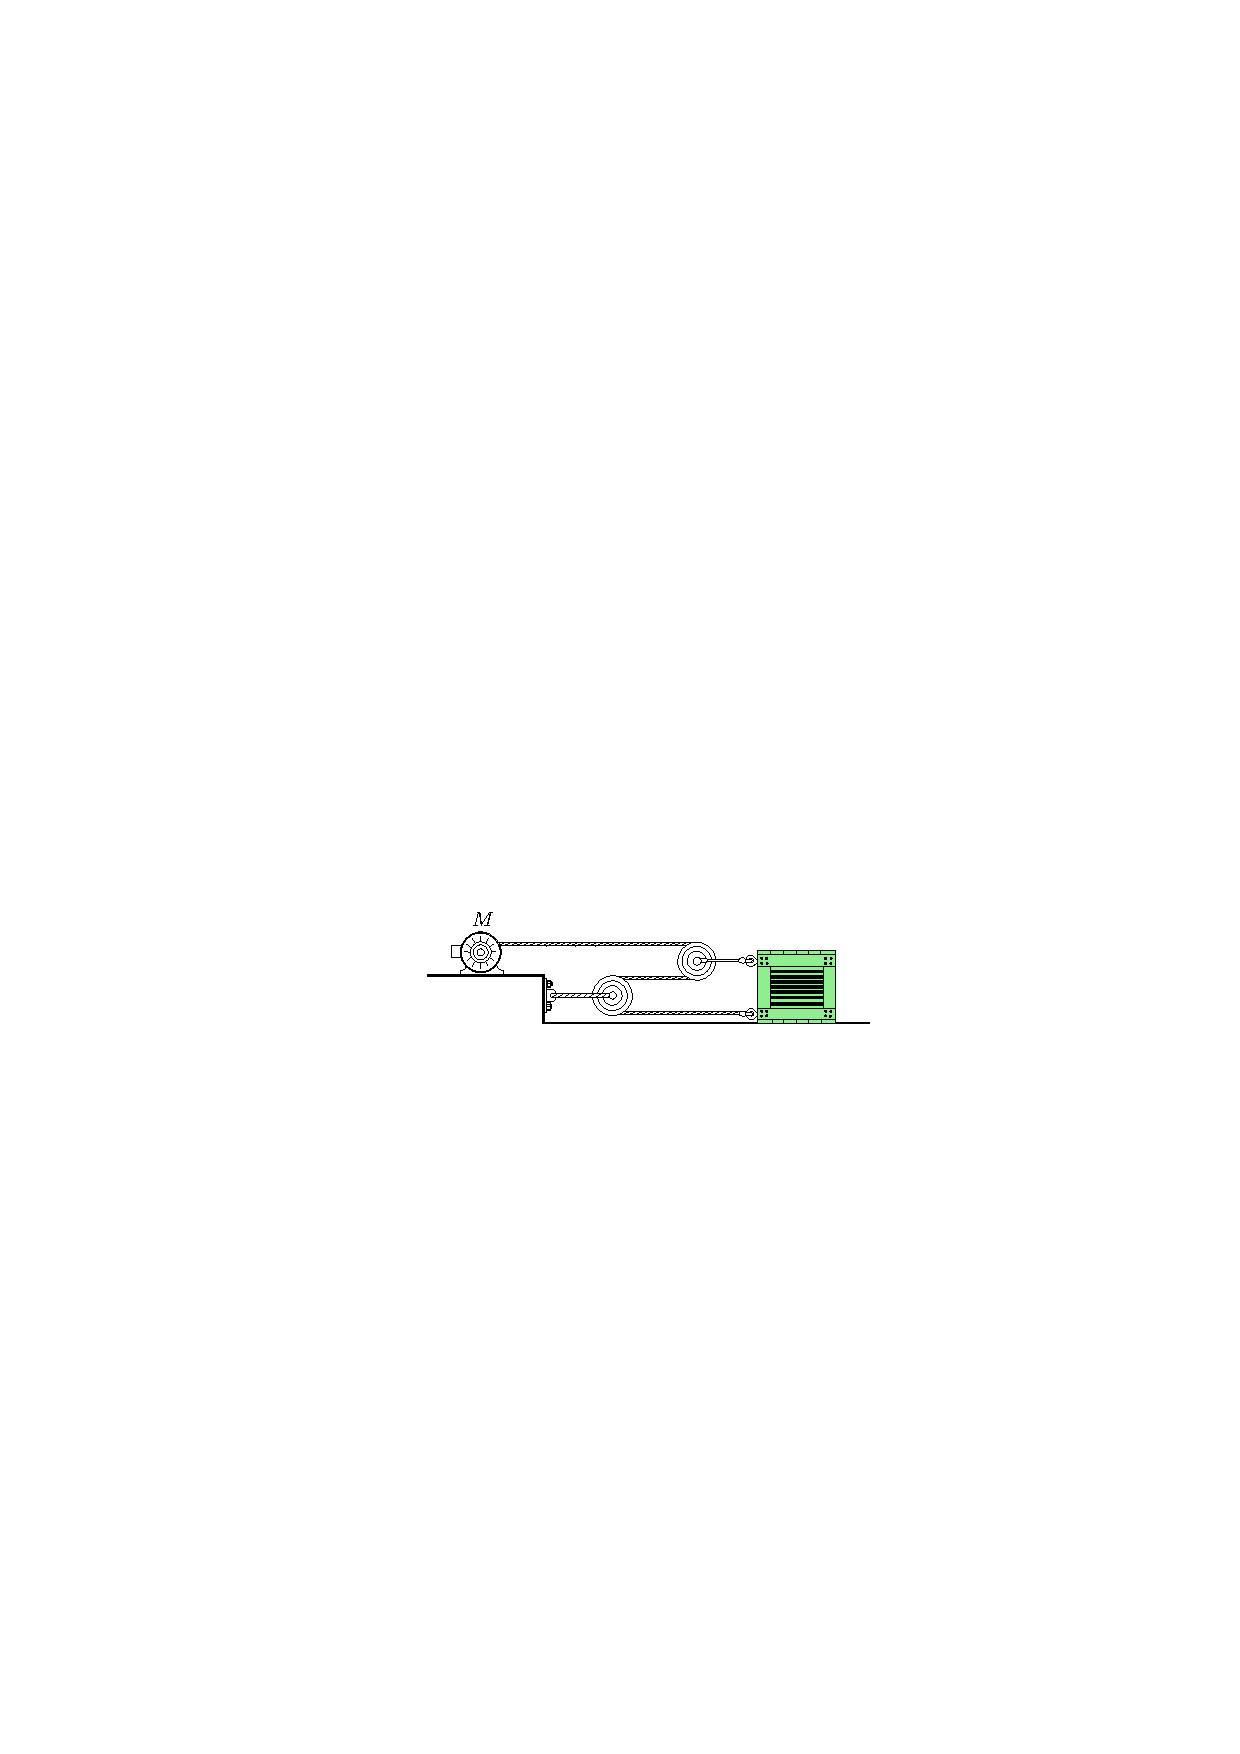
\includegraphics[scale=2]{images/draw_9.pdf}
\end{flushleft}